\documentclass[pdf,aspectratio=169]{beamer}
\usepackage[]{hyperref,graphicx,siunitx,booktabs,lmodern}
\usepackage{physics}
\usepackage{em-commands}
\mode<presentation>{\usetheme{EM}}

%Question Numbering
\newcounter{questionnumber}
\newcommand{\qnum}{%
	\stepcounter{questionnumber}%
	Q\arabic{questionnumber}
}
\resetcounteronoverlays{questionnumber}

\graphicspath{ {../Images/} }

\sisetup{per-mode=symbol}

\tikzstyle{plate}=[draw, very thick, minimum width=4cm, minimum height=1cm, fill=gray!40, anchor=south]

%preamble
\title{Susceptible Lines}
\date{November 16, 2018}
\author{Jed Rembold}

\begin{document}
\renewcommand{\theenumi}{\Alph{enumi}}

\begin{frame}{Announcements}
	\begin{itemize}
		\item Homework
			\begin{itemize}
				\item Homework 11 has been posted
				\item Due Wednesday night after break
				\item All Ch 6 material (and maybe a smidge of 5)
			\end{itemize}
		\item Physics Tea at 3!
		\item Don't forget to wow your family with E\&M knowledge over dinner next Thursday!
			\begin{itemize}
				\item I will actually throw some extra credit toward your worst test score if you film yourself explaining some E\&M concept to a clueless family member or friend. Say a 1-3 minute explanation!
			\end{itemize}
			
	\end{itemize}
\end{frame}

\begin{frame}{\qnum}
	We defined the polarizability in terms of the $\ef$:
	\[\pol = \epsilon_0 \chi_e \ef\]
	Yet we define the magnetization in terms of $\af$:
	\[\vmag = \chi_m \af\]
	Why?
	\begin{enumerate}
		\item It is different physics. The magnetization actually depends only on $\af$.
		\item \alert<2>{It is easier to measure quantities related to $\af$ in the lab.}
		\item It is more convenient algebraically to write it this way.
		\item It is simply an old tradition like calling the current the direction that positive charges flow.
	\end{enumerate}
\end{frame}


\begin{frame}{\qnum}
	For linearly magnetizable materials, the relationship between the magnetization and the H-field is
	\[\vmag = \chi_m \af\]
	What do you expect the sign of $\chi_m$ to be for a paramagnetic/diamagnetic material?
	\begin{enumerate}
		\item Both positive
		\item Both negative
		\item \alert<2>{Para positive and Dia negative}
		\item Para negative and Dia positive
	\end{enumerate}
\end{frame}

\begin{frame}{\qnum}
	A \SI{100}{\ampere} current is measured running through a \SI{10}{\milli\meter} diameter copper wire. What is the magnetic field halfway from the center to the outer edge?
	\begin{enumerate}
		\item \SI{999.99}{\micro\tesla}
		\item \alert<2>{\SI{1999.98}{\micro\tesla}}
		\item \SI{3999.96}{\micro\tesla}
		\item \SI{4000}{\micro\tesla}
	\end{enumerate}
\end{frame}

\begin{frame}[fragile]{\qnum}
	\newcommand{\ferro}[4]{
		\begin{scope}
			\clip (#1) rectangle +(#2);
			\fill[#4!50!black!50] (0,0) rectangle +(4,3);
			\foreach \x in {0,.4,...,4}{
				\foreach \y in {0,.4,...,3}{
					\draw[thick, -latex] (\x,\y) -- +(#3:.3);
				}
			}
		\end{scope}
	}
	\begin{columns}
		\column{0.5\textwidth}
		A ferromagnet has domains with dipoles moments as indicated to the right. After being placed in a magnetic field which points in the upward direction, which image below best depicts the ferromagnet?
		\column{0.5\textwidth}
		\begin{center}
			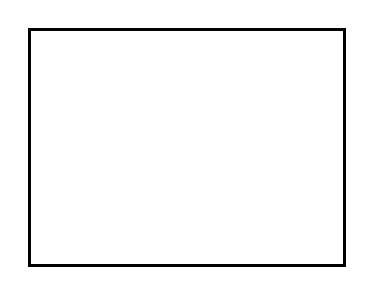
\begin{tikzpicture}
				\ferro{4,3}{-2,-1.5}{180}{orange}
				\ferro{0,3}{2,-1.5}{90}{cyan}
				\ferro{0,0}{2,1.5}{0}{yellow}
				\ferro{4,0}{-2,1.5}{-90}{violet}
				\draw[very thick] (0,0) rectangle +(4,3);
			\end{tikzpicture}
		\end{center}
	\end{columns}
	\begin{center}
		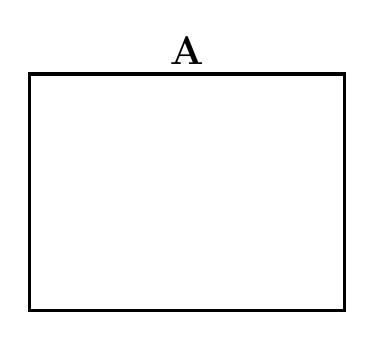
\begin{tikzpicture}
			\ferro{4,3}{-2,-1.5}{90}{orange}
			\ferro{0,3}{2,-1.5}{90}{cyan}
			\ferro{0,0}{2,1.5}{90}{yellow}
			\ferro{4,0}{-2,1.5}{90}{violet}
			\draw[very thick] (0,0) rectangle +(4,3);
			\node[font=\Large\bf,above] at (2,3) {A};
		\end{tikzpicture}
		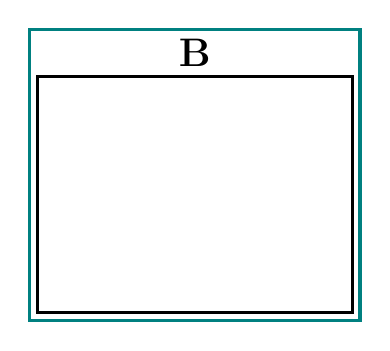
\begin{tikzpicture}
			\ferro{4,3}{-2,-1.5}{180}{orange}
			\ferro{0,0}{2,1.5}{0}{yellow}
			\ferro{4,0}{-2,1.5}{-90}{violet}
			\ferro{0,3}{3,-2.0}{90}{cyan}
			\draw[very thick] (0,0) rectangle +(4,3);
			\node[font=\Large\bf,above] at (2,3) {B};
			\draw<2>[very thick, teal] (-.1,-.1) rectangle +(4.2,3.7);
		\end{tikzpicture}
		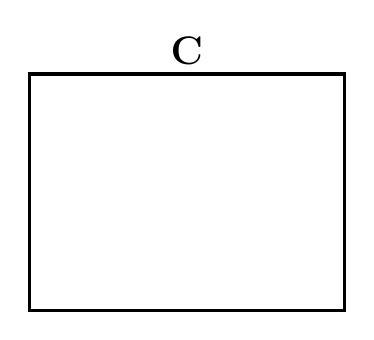
\begin{tikzpicture}
			\ferro{4,3}{-2,-1.5}{90}{orange}
			\ferro{0,0}{2,1.5}{90}{yellow}
			\ferro{4,0}{-2,1.5}{90}{violet}
			\ferro{0,3}{3,-2.0}{90}{cyan}
			\draw[very thick] (0,0) rectangle +(4,3);
			\node[font=\Large\bf,above] at (2,3) {C};
		\end{tikzpicture}
	\end{center}
\end{frame}

\begin{frame}{\qnum}
	\begin{columns}
		\column{0.5\textwidth}
		The image to the right is a hysteresis loop for a ferromagnetic material with a current carrying wire wrapped about it. As the current is turned from positive to negative and back, what direction does one travel around the loop?
		\begin{enumerate}
			\item Clockwise
			\item \alert<2>{Counterclockwise}
			\item It depends on other factors
		\end{enumerate}
		
		\column{0.5\textwidth}
		\begin{center}
			\begin{tikzpicture}
				\draw[very thick, fill=teal!20]
					(-3,-3) .. controls +(0:5) and +(180:2) .. (3,3)
					.. controls +(180:5) and +(0:2) .. (-3,-3);
				\draw<2>[very thick, fill=teal!20, ->>-=0.2 to .9 by .2]
					(-3,-3) .. controls +(0:5) and +(180:2) .. (3,3)
					.. controls +(180:5) and +(0:2) .. (-3,-3);
				\path[thick, -latex] 
					(-3,0) edge node[at end,right,math] {\mcur} (3,0)
					(0,-3) edge node[at end,above,math] {M} (0,3);
			\end{tikzpicture}
		\end{center}
	\end{columns}
\end{frame}

%\begin{frame}{\qnum}
	%\begin{columns}
		%\column{0.5\textwidth}
		%\begin{center}
			%\begin{tikzpicture}
				%\draw[very thick, fill=violet!20, name path=cv]
					%(-3,-3) .. controls +(0:5) and +(180:2) .. (3,3)
					%.. controls +(180:5) and +(0:2) .. (-3,-3);
				%\path[thick, -latex] 
					%(-3,0) edge node[at end,right,math] {H} (3,0)
					%(0,-3) edge node[at end,above,math] {B} (0,3);
				%\path[name path=y] (0,-3) -- (0,3);
				%\node[name intersections={of=cv and y, by=p}, point] at (p) {};
			%\end{tikzpicture}
		%\end{center}
		
		%\column{0.5\textwidth}
		%Given the hysteresis curve to the left, what can be stated about the indicated point?
		%\begin{enumerate}
			%\item No magnetic field is being applied to the ferromagnet
			%\item The ferromagnet currently has 0 permanent magnetization
			%\item Increasing the applied magnetic field will increase the magnitude of the ferromagnet's magnetic field
			%\item A negative magnetic field is being applied to the ferromagnet
		%\end{enumerate}
		
	%\end{columns}
%\end{frame}

%\begin{frame}{\qnum}
	%What are the units for the area under a $\af$-$\mf$ hysteresis curve?
	%\begin{enumerate}
		%\item $\displaystyle\si[per-mode=fraction]{\square\tesla \ampere\per\newton}$
		%\item $\displaystyle\si[per-mode=fraction]{\newton\per\square\meter}$
		%\item $\displaystyle\si[per-mode=fraction]{\square\tesla}$
		%\item $\displaystyle\si[per-mode=fraction]{\tesla\ampere\per\square\newton}$
	%\end{enumerate}
%\end{frame}







\end{document}
